\documentclass{article}

% Language setting
% Replace `english' with e.g. `spanish' to change the document language
\usepackage[english]{babel}

% Other packages that are useful for math
\usepackage{amssymb}
\usepackage{amsmath}

% Set page size and margins
% Replace `letterpaper' with `a4paper' for UK/EU standard size
\usepackage[letterpaper,top=2cm,bottom=2cm,left=3cm,right=3cm,marginparwidth=1.75cm]{geometry}

\usepackage{listings}
\usepackage{color}

\definecolor{dkgreen}{rgb}{0,0.6,0}
\definecolor{gray}{rgb}{0.5,0.5,0.5}
\definecolor{mauve}{rgb}{0.58,0,0.82}

\lstset{frame=tb,
  language=Python,
  aboveskip=3mm,
  belowskip=3mm,
  showstringspaces=false,
  columns=flexible,
  basicstyle={\small\ttfamily},
  numbers=none,
  numberstyle=\tiny\color{gray},
  keywordstyle=\color{blue},
  commentstyle=\color{dkgreen},
  stringstyle=\color{mauve},
  breaklines=true,
  breakatwhitespace=true,
  tabsize=3
}

% Useful packages
\usepackage{amsmath}
\usepackage{graphicx}
\usepackage[colorlinks=true, allcolors=blue]{hyperref}

\title{Zombie Apocalypses in the Media: Epidemic Modeling in HBO's \textit{The Last of Us (2023)}}
\author{Andrew Antenberg, Caia Gelli, Caylen David, Campbell Phalen, \& Lily Goldstein}

\begin{document}
\maketitle

\begin{abstract}
Since the inception of the cinema, film and television have provided audiences entertainment that offers a vision at both near and distant visions of the world. One form of media that typically suspend the audience's disbelief. Within the media genre of zombie apocalypses, we seek to base these types of media in reality through outbreak and epidemic modeling. In our paper, we will outline some commons zombie outbreak models that are based in SIR epidemic modeling, while also introducing our own model that takes the SIR model to a more nuanced level through examining how differentiated survival strategies affect infection and death rates. After an attempt at using linear stability to determine equilibra and the model's stability, we will discuss the results of a simulation of our model that forecasts our model until the exinction of humanity. We will compare our results to the world depicted in HBO's \textit{The Last of Us (2023)}, ultimately showing that the apocalyptic environment within the piece of media reflects the findings in our model and simulation. 
\end{abstract}

\section{Introduction}

In epidemiology, mathematical models provide valuable tools for understanding the spread and dynamics of infectious diseases. The original model for the zombie apocalypse that inspired our own, is based on the SIR model. The SIR model is a compartmental model that divides a population into three main compartments based on their disease status: susceptible, infected and removed. Susceptible individuals are those at risk of contracting the disease, Infected individuals are currently infected and possibly able to transmit the disease to others, and removed individuals are those who are immune or no longer infectious. This basic model assumes that individuals can only transition between these three compartments.

From this setup, we are able to consider several factors to develop the rates of traffic between these classes, i.e. rates of transmission, infection, and recovery. These rates are influenced by several factors, including the infectiousness of the disease, contact rate between classes, recovery rate, and risk of re-infection. With these factors, we are able to formulate the SIR model as a set of differential equations that quantify the rates of change of the population sizes of each class.

After setting up the model, the next step is to conduct linear stability analysis on the system to determine whether small perturbations around an equilibrium point will grow or decay over time. We employ this method by forming the Jacobian matrix, which provides a local linear approximation of the system’s behavior near an equilibrium point. The Jacobian Matrix is a Matrix of partial derivatives that describes the sensitivity of the rates of change of the variables to infinitesimal changes in the variables themselves. Thus, to construct the Jacobian for the SIR model you take the partial derivatives of the rate equations with respect to S, I and R.

Following this, we compute the eigenvalues of the Jacobian matrix. The eigenvalues capture the rate at which perturbations grow or decay around the equilibrium point. If the eigenvalues for a particular equilibrium point have negative real parts, the equilibrium point is considered to be linearly stable. This indicates that perturbations around the equilibrium point will decay over time. On the other hand, if there exists an eigenvalue with a positive real part, the equilibrium point is unstable. In this case, perturbations around the equilibrium point will amplify over time.

\section{The Basic Model}

The paper ``When Zombies Attack!: Mathematical Modeling of an Outbreak of Zombie Infection” provides the basic model for tracking the evolution of a zombie epidemic. The basic model that this paper introduces considers three basic classes: Susceptibles (\emph{S}), Zombies (\emph{Z}), and Removed (\emph{R}) \cite{zombies}. Susceptibles are healthy humans that have not yet been infected. They can become deceased through natural causes (parameter $\delta$) and enter class \emph{R}, or they can become a zombie (parameter $\beta$) and enter class \emph{Z}. If a zombie is killed (parameter $\alpha$), they enter class \emph{R}. Lastly, deceased humans in class \emph{R} can be resurrected as a zombie (parameter $\zeta$), and enter class \emph{Z}. This model assumes that the birth rate, $\Pi$ is constant. Using these parameters, the equations for the model are as follows:
\begin{align*}
S' &= \Pi - \beta SZ - \delta S \\
Z' &= \beta SZ + \zeta R - \alpha S Z \\
R' &= \delta S + \alpha SZ - \zeta R
\end{align*}
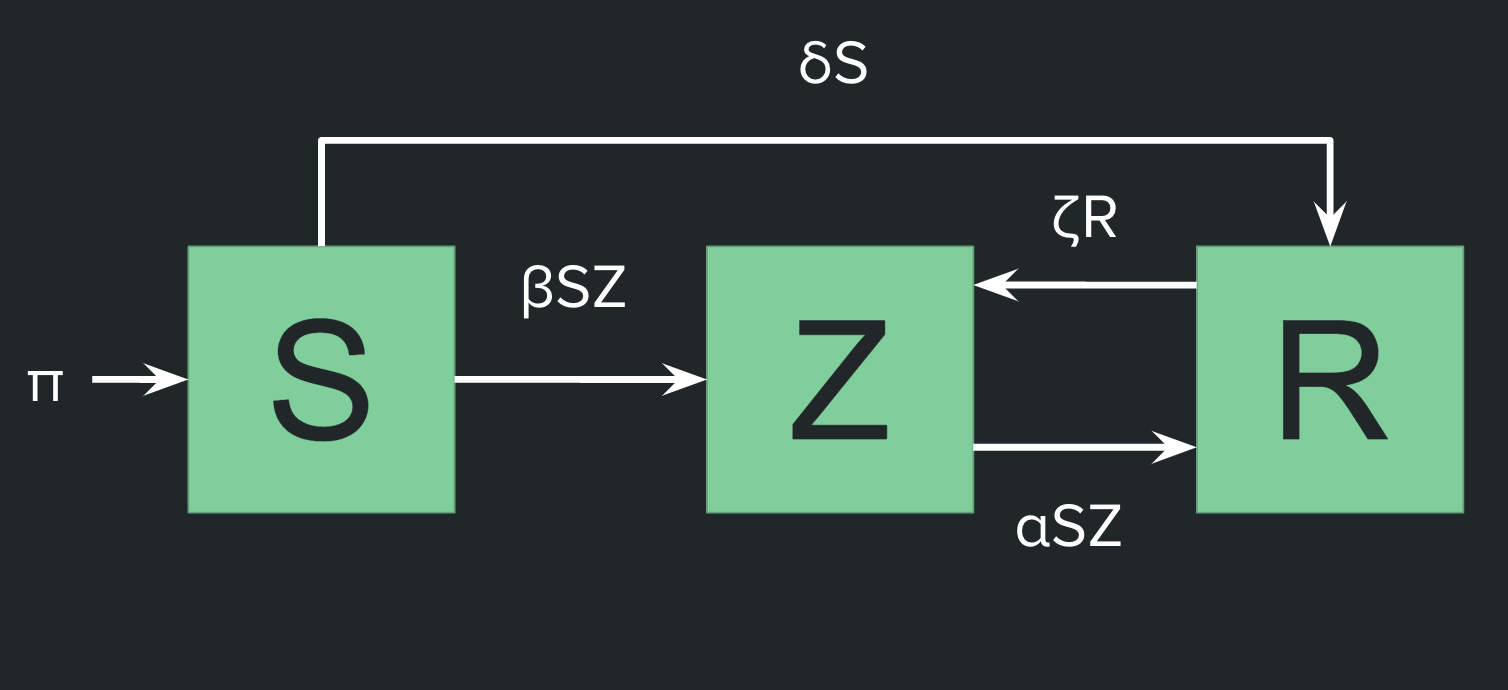
\includegraphics[width=1\textwidth]{SZR Model.png}\\
\\
After defining this model, the authors' goal was to determine if a stable equilibrium point exists such that zombies and uninfected humans can both exist. They assumed the outbreak takes place over a short timescale, thus ignoring birth and background death rates. The two equilibrium points found were at $\emph{Z}=0$, the disease free equilibrium, and at $\emph{S}=0$, the "doomsday" equilibrium, where all people are either zombies or dead. These equilibrium points show that the coexistence of humans and zombies is impossible. However, they found that the disease-free equilibrium is unstable, as the only equilibrium point with a Jacobian with all negative eigenvalues occurs at the doomsday equilibrium. In other words, in a zombie outbreak, zombies will likely infect everyone, and there would be no Susceptibles remaining.

\section{Mathematical Shortcomings of ``When Zombies Attack!"}
For the majority of the models analyzed in ``When Zombies Attack!", the paper concludes that the only stable equilibria are at the extremes, where the entire population ends up in one group. When searching for linear stable equilibria, ``When Zombies Attack!" uses perturbations in 3 dimensions, because the SZR model has three variables. However, it is important to note that without a birth rate, the sum of the populations of the three groups must be constant. Thus, the problem is really two-dimensional, not three-dimensional. Using three-dimensional perturbations causes analysis to miss equilibrium points that are linearly stable in two dimensions. We will perform analysis on the SZR in two dimensions following math from Ted Chinburg's 2020 paper, ``Epidemics with Renewed Susceptibility."

We begin by defining the rates of change in the populations of the susceptible, zombie, and removed groups with the following equations:
\begin{align*}
    \frac{\mathrm{dS}}{\mathrm{dt}} &= -\alpha S Z + \delta R \\
    \frac{\mathrm{dZ}}{\mathrm{dt}} &= \alpha S Z - \tau Z \\
    \frac{\mathrm{dR}}{\mathrm{dt}} &= \tau Z - \delta Z  
\end{align*}
We can normalize the time unit such that $\tau = 1$, and normalize the population to be 1. Doing so, we can eliminate $R$ because $R = 1 - S - Z$. This allows us to express the flow rates in just two equations:
\begin{align*}
    \frac{\mathrm{dS}}{\mathrm{dt}} &= -\alpha S Z + \delta (1-S-Z) \\
    \frac{\mathrm{dZ}}{\mathrm{dt}} &= \alpha S Z - Z
\end{align*}
To find linear stability, we replace the equations with their first order Taylor approximation and look for stability. To do this, we look for points where $\frac{\mathrm{dS}}{\mathrm{dt}} = \frac{\mathrm{dZ}}{\mathrm{dt}} = 0$ and the eigenvalues of the Jacobian matrix of this equations have negative real parts. In the case where $\delta > 0$ and $\alpha > 1$, equilibrium points exist at $$(S(0), Z(0)) = (\frac{1}{\alpha}, (1-\frac{1}{\alpha})/(\frac{1}{\delta} + 1)$$

Analyzing these equations in two dimensions allows us to find non-extreme equilibria under some specific conditions. This conclusion was overlooked by ``When Zombies Attack!" and inspired us to try to analyze more complex models.

\section{The Last of Us (TLOU) Model}

\subsection{Introduction to \textit{The Last Of Us (2023)}}

For our project, the piece of post-apocalyptic media that we will be modeling is that of \textit{The Last of Us (2023)}, a popular television series on HBO Max based off of the popular 2013 video game of the same name. A large aspect of this series focuses on the human monsters that live in a post-apocalyptic society in addition to the Zombies that walk the Earth. This reflects a key distinction that we wish to explore within our model: The fact that individuals living in a zombie apocalypse react differently, employing different survival methods that consequently affect death rates and transmission rates.

The zombie pandemic presented in \textit{The Last of Us} presents a mutated version of the Cordyceps fungus. This fungus is a parasitic mind-controlling fungus, commonly referred to as the "zombie-ant fungus". Within nature, the fungus parasitizes the brain of insects, taking control of their mind while preserving the body of the controlled insect. This allows for an organism to become "zombified" without their body decomposing. Within \textit{The Last of Us}, rising global temperatures caused the Cordyceps fungus to mutate and infect humans through an identical framework. The fungus controls the infected zombie "puppets" through a hive-mind mentality, and since the bodies are preserved by the fungus, zombies live forever unless killed by a human.

\subsection{Setting Up TLOU Model}

Figure 1 illustrates our model. For the model, the key distinction from other zombie epidemic models is the division of \textbf{Susceptibles (S)} into three subclasses:

\begin{itemize}
    \item Raiders ($S_R$)
    \item Survivalists ($S_S$)
    \item Civilians ($S_C$)
\end{itemize}

Raiders are aggressive gang factions that adopt a "survival of the fittest" mentality. They are the most adequately equipped against the zombie outbreak, and they are also willing to kill other Susceptibles to usurp their resources and remain dominant. The Raiders represent the "Human Monsters" that exist within the world of \textit{The Last of Us}.

Survivalists live alone or in very small groups. They are nomads, frequently traveling and looking to minimize all contact, both with other Susceptibles and Zombies.

Civilians are essentially the opposite of Raiders. They represent those who unite together after the shock of the apocalypse, but not in an aggressive way. Rather, the Civilians represent those who have united to maintain some level of post-apocalyptic societal structure. They are poorly armed, and least likely to fight against the Raiders and Zombies, but they also have the fortifications and infrastructure to prolong their operations and live through collaboration and sharing of resources. 

Susceptibles can become deceased through 'natural' causes, i.e. non-zombie-related deaths, including dying from other Susceptible factions (Death Parameter $\delta_1$ , $\delta_2$ , and $\delta_3$ , representing the death rates for Raiders, Survivalists, and Civilians respectively). Susceptibles deceased through non-zombie-related death become part of the \textbf{Removed (R)} class. Susceptibles may also jump between subclasses, with the Survivalists serving as the middle man—A Civilian may eventually become a Raider, and vice versa, but not before becoming part of the Survivalist class. These class exchange rates are represented by: 

\begin{itemize}
    \item $\epsilon_{1,2}$ : Parameter representing the exchange rate from Raider to Survivalist.
    \item $\epsilon_{2,1}$ : Parameter representing the exchange rate from Survivalist to Raider.
    \item $\epsilon_{2,3}$ : Parameter representing the exchange rate from Survivalist to Civilian.
    \item $\epsilon_{3,2}$ : Parameter representing the exchange rate from Civilian to Survivalist. 
\end{itemize}

Susceptibles can become a \textbf{Zombie (Z)} through transmission via a "lost" encounter with a zombie (Transmission parameters $\zeta_1$ , $\zeta_2$ , and $\zeta_3$, representing the transmission rates for Raiders, Survivalists, and Civilians respectively). A key feature that our model includes from \textit{The Last of Us} is that due to the Cordyceps virus preserving the body of a Zombie, rendering it as a zombified puppet in perpetuity, zombies live forever in our model unless killed by a Susceptible. We also assume that zombies do not kill other zombies, and they only attack Susceptibles who have the opportunity to become infected.

The \textbf{Removed (R)} class includes Susceptibles killed through non-zombie-related, as well as zombies that are killed by Susceptibles ("Headshot" Parameter $\sigma$ , representing the death rate of Zombies who have "lost" an encounter with a Susceptible). Since the mind-controlling Cordyceps are reliant on preserving the fertility of the body of those they zombify, there is no resurrection once Susceptibles or Zombies are deceased. We also assume that there is a birth rate that is a constant, $\Pi$. We will assume that there is a constant birth rate among each subclass.

Thus, the basic model is given by: 
\begin{align*}
    S_R' &= \Pi/3 + \epsilon_{2,1}S_RS_S - \epsilon_{1,2}S_RS_S - \delta_1S_R - \zeta_1S_RZ \\
S_S' &= \Pi/3 + \epsilon_{1,2}S_RS_S + \epsilon_{3,2}S_SS_C - \epsilon_{2,1}S_RS_S - \epsilon_{2,3}S_SS_C - \delta_2S_S - \zeta_2S_SZ\\
S_C' &= \Pi/3 + \epsilon_{2,3}S_SS_C - \epsilon_{3,2}S_SS_C - \delta_3S_C - \zeta_3S_CZ\\
Z' &= \zeta_1S_RZ + \zeta_2S_SZ + \zeta_3S_CZ
\end{align*}

With our entire population subject to the constraint:

$$S_R + S_S + S_C + Z = C$$

Where \textbf{C} represents the entire population who is alive, either as a Susceptible or a Zombie. When conducting our linear stability analysis, we assume that the birth rate equals the death rate for $S_R$ , $S_S$ , and $S_C$. Additionally, zombies live forever unless killed, and cannot be resurrected from the dead. Both of these conditions render the environment as a closed system from which we will conduct our equilibria analysis. With this, our system of differential equations becomes: 




\begin{figure}
\centering
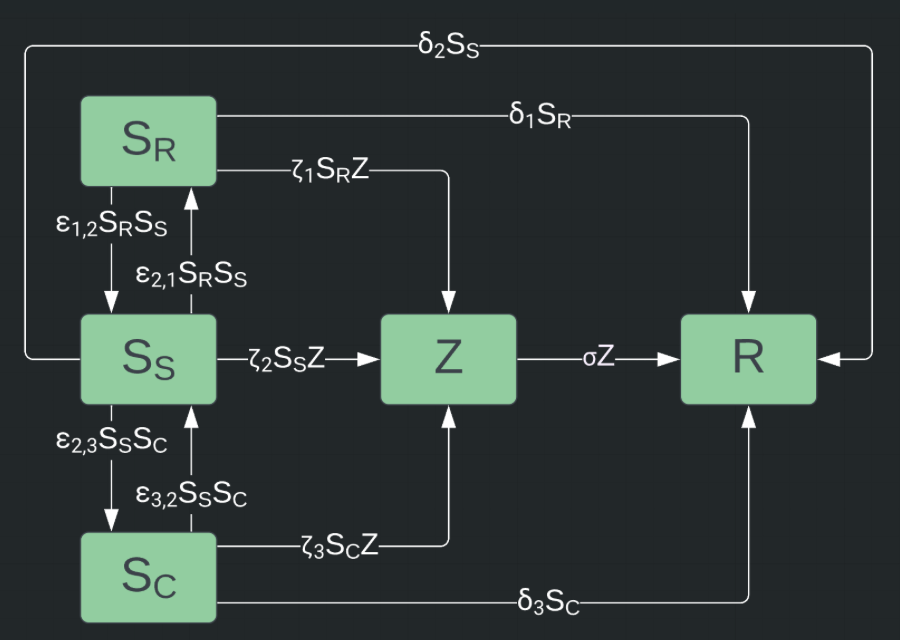
\includegraphics[width=1\textwidth]{TLOU Model Outline.png}
\caption{\label{fig:frog} The Last of Us (TLOU) Model}
\end{figure}

\subsection{TLOU Equilibria Analysis}

Observe that
\begin{align*}
    S_R' &= \epsilon_{2,1} S_R S_S - \epsilon_{1,2} S_R S_S - \delta_1 S_R - \zeta_1 S_R Z \\
    S_S' &= \epsilon_{1,2} S_R S_S + \epsilon_{3,2} S_S S_C - \epsilon_{2,1} S_R S_S - \epsilon_{2,3} S_S S_C - \delta_2 S_S - \zeta_2 S_S Z \\
    S_C' &= \epsilon_{2,3} S_S S_C - \epsilon_{3,2} S_S S_C - \delta_3 S_C - \zeta_3 S_S Z \\
    Z'   &= \zeta_1 S_R Z + \zeta_2 S_S Z + \zeta_3 S_C Z \\
    C    &= S_R + S_S + S_C + Z
\end{align*}
where $C$ is some constant representing the sum of all populations. Because there is no birth rate and no death rate, $C$ will be constant. In an equilibrium state, we would see
\[
    \begin{pmatrix}
    \epsilon_{2,1} S_R S_S - \epsilon_{1,2} S_R S_S - \delta_1 S_R - \zeta_1 S_R Z \\
    \epsilon_{1,2} S_R S_S + \epsilon_{3,2} S_S S_C - \epsilon_{2,1} S_R S_S - \epsilon_{2,3} S_S S_C - \delta_2 S_S - \zeta_2 S_S Z \\
    \epsilon_{2,3} S_S S_C - \epsilon_{3,2} S_S S_C - \delta_3 S_C - \zeta_3 S_C Z \\
    \zeta_1 S_R Z + \zeta_2 S_S Z + \zeta_3 S_C Z \\
    S_R + S_S + S_C + Z
    \end{pmatrix}
    =
    \begin{pmatrix}
        0 \\
        0 \\
        0 \\
        0 \\
        C
    \end{pmatrix}
\]
Solving this system of equations yields a number of non-trivial solutions
\[
    S_R + S_c = C,\, S_S = 0,\, Z = 0
\]
In this equilibrium is when all the population is split between the raiders and the citizens, the zombies are eradicated though.
\[
    S_R = 0,\, S_S = C,\, S_c = 0,\, Z = 0 
\]
For this equilibrium, all of the population falls into the survivalist group, the zombies are again eradicated.
\[
    S_R = 0,\, S_S = 0,\, S_c = 0,\, Z = C
\]
Here, the entire population is infected and become zombies.
\[
    S_R = \frac{C \zeta_2}{\epsilon_{1,2} - \epsilon_{2,1} - \zeta_1 + \zeta_2},\,
    S_S = \frac{C \zeta_1}{-\epsilon_{1,2} + \epsilon_{2,1} + \zeta_1 - \zeta_2},\,
    S_C = 0,\,
    Z = \frac{C (\epsilon_{1,2} - \epsilon_{2,1})}{\epsilon_{1,2} - \epsilon_{2,1} - \zeta_1 + \zeta_2}
\]
Perhaps a more intruiging equilibrium, population is split between raider, survivalist, and zombie populations. However, this is actually an invalid equilibrium because it does not match the constraint that $S_R, S_S, S_C, Z \geq 0$. To demonstrate this, observe that the denominator for $S_R$ is
\[
    \epsilon_{1,2} - \epsilon_{2,1} - \zeta_1 + \zeta_2
\]
while the demoninator for $S_S$ is
\[
    -\epsilon_{1,2} + \epsilon_{2,1} + \zeta_1 - \zeta_2
\]
because these are additive inverse, we know that one must be positive and the other negative. Therefore one of $S_R$ or $S_S$ must be negative, meaning we break the constraint of all populations being positive.
\[
    S_R = \frac{C \zeta_3}{\zeta_3 - \zeta_1},\,
    S_S = 0,\,
    S_C = \frac{C \zeta_1}{\zeta_1 - \zeta_3},\,
    Z = 0
\]
This next equilibrium has the same issue, $\zeta_3 - \zeta_1$ and $\zeta_1 - \zeta_3$ are additive inverses so one must be negative, resulting in $S_R$ or $S_C$ being negative.
\[
    S_R = \frac{C (\epsilon_{2,3} - \epsilon_{3,2})}{\epsilon_{1,2} - \epsilon_{2,1} + \epsilon_{2,3} - \epsilon_{3,2}},\,
    S_S = 0,\,
    S_C = \frac{C (\epsilon_{1,2} - \epsilon_{2,1})}{\epsilon_{1,2} - \epsilon_{2,1} + \epsilon_{2,3} - \epsilon_{3,2}},\,
    Z = 0
\]
which is our final equilibrium that is valid (for certain values of $\epsilon_{1,2}, \epsilon_{2, 1}, \epsilon_{2, 3}, \epsilon_{3, 2}$). 

Now for stability analysis. The Jacobian will be
\[
    \resizebox{\linewidth}{!}{%
    $\displaystyle
    \begin{pmatrix}
        \epsilon_{2, 1} S_S - \epsilon_{1, 2} S_S - \delta_1 - \zeta_1 Z & \epsilon_{2, 1} S_R - \epsilon_{1, 2} S_R & 0 & \zeta_1 S_R \\
        \epsilon_{1, 2} S_S - \epsilon_{2, 1} S_S & \epsilon_{1, 2} S_R + \epsilon_{3, 2} S_C - \epsilon_{2, 1} S_R - \epsilon_{2, 3} S_C - \delta_2 - \zeta_2 Z & \epsilon_{3, 2} S_S - \epsilon_{3, 2} S_S & \zeta_2 S_S \\
        0 & \epsilon_{2, 3} S_C - \epsilon_{3, 2} S_C & \epsilon_{2, 3} S_S - \epsilon_{3, 2} S_S - \delta_3 - \zeta_3 Z & \zeta_3 S_C \\
        \zeta_1 Z & \zeta_2 Z & \zeta_3 Z & \zeta_1 S_R + \zeta_2 S_S + \zeta_3 S_C
    \end{pmatrix}
    $}
\]
Plugging in
\[
    S_R = \frac{C (\epsilon_{2,3} - \epsilon_{3,2})}{\epsilon_{1,2} - \epsilon_{2,1} + \epsilon_{2,3} - \epsilon_{3,2}},\,
    S_S = 0,\,
    S_C = \frac{C (\epsilon_{1,2} - \epsilon_{2,1})}{\epsilon_{1,2} - \epsilon_{2,1} + \epsilon_{2,3} - \epsilon_{3,2}},\,
    Z = 0
\]
we have
\[
    \begin{pmatrix}
        \delta_1 - \zeta_1 Z & \epsilon_{2, 1} S_R - \epsilon_{1, 2} S_R & 0 & \zeta_1 S_R \\
        0 & \epsilon_{1, 2} S_R + \epsilon_{3, 2} S_C - \epsilon_{2, 1} S_R - \epsilon_{2, 3} S_C - \delta_2 - \zeta_2 Z & 0 & 0 \\
        0 & \epsilon_{2, 3} S_C - \epsilon_{3, 2} S_C & \delta_3 - \zeta_3 Z & \zeta_3 S_C \\
        \zeta_1 Z & \zeta_2 Z & \zeta_3 Z & \zeta_1 S_R + \zeta_3 S_C
    \end{pmatrix}
\]
which further simplifies to
\[
    \begin{pmatrix}
        - \delta_1 & \frac{C (\epsilon_{1, 2} - \epsilon_{2, 1})(\epsilon_{2,3} - \epsilon_{3,2})}{\epsilon_{1,2} - \epsilon_{2,1} + \epsilon_{2,3} - \epsilon_{3,2}} & 0 & \frac{C \zeta_1 (\epsilon_{2,3} - \epsilon_{3,2})}{\epsilon_{1,2} - \epsilon_{2,1} + \epsilon_{2,3} - \epsilon_{3,2}} \\
        0 & \frac{2 C (\epsilon_{1, 2} - \epsilon_{2, 1})(\epsilon_{2,3} - \epsilon_{3,2})}{\epsilon_{1,2} - \epsilon_{2,1} + \epsilon_{2,3} - \epsilon_{3,2}} - \delta_2 & 0 & 0\\
        0 & \frac{C (\epsilon_{1, 2} - \epsilon_{2, 1})(\epsilon_{2,3} - \epsilon_{3,2})}{\epsilon_{1,2} - \epsilon_{2,1} + \epsilon_{2,3} - \epsilon_{3,2}} & - \delta_3 & \frac{C \zeta_3 (\epsilon_{1,2} - \epsilon_{2,1})}{\epsilon_{1,2} - \epsilon_{2,1} + \epsilon_{2,3} - \epsilon_{3,2}} \\
        0 & 0 & 0 & C \cdot \frac{\zeta_1 (\epsilon_{1, 2} - \epsilon_{2, 1}) + \zeta_3 (\epsilon_{2,3} - \epsilon_{3,2})}{\epsilon_{1,2} - \epsilon_{2,1} + \epsilon_{2,3} - \epsilon_{3,2}}
    \end{pmatrix}
\]
this matrix has eigenvalues
\[
    \lambda_1 = -\delta_1,
\]
\[
    \lambda_2 = -\delta_3,
\]
\[
    \lambda_3 = \frac{-\delta_2 \epsilon_{1,2} + \delta_2 \epsilon_{2,1} - \delta_2 \epsilon_{2,3} + 2 C \epsilon_{1,2} \epsilon_{2,3} - 2 C \epsilon_{2,1} \epsilon_{2,3} + \delta_2 \epsilon_{3,2} - 2 C \epsilon_{1,2} \epsilon_{3,2} + 2 C \epsilon_{2,1} \epsilon_{3,2}}{\epsilon_{1,2} - \epsilon_{2,1} + \epsilon_{2,3} - \epsilon_{3,2}},
\]
\[
    \lambda_4 = \frac{C (\epsilon_{1,2} \zeta_1 - \epsilon_{2,1} \zeta_1 + \epsilon_{2,3} \zeta_3 - \epsilon_{3,2} \zeta_3)}{\epsilon_{1,2} - \epsilon_{2,1} + \epsilon_{2,3} - \epsilon_{3,2}}
\]
Now we are curious as to when these eigenvalues can be all negative. Let's say $\delta_1 = \delta_3 = 1$, this yields that our first two eigenvalues, $\lambda_1, \lambda_2$ are negative. Next, we can set $\zeta_1 = \zeta_3 = -1$ and eigenvalue four simplifies down to
\begin{align*}
    \lambda_4 &=
    \frac{C (\epsilon_{1,2} \zeta_1 - \epsilon_{2,1} \zeta_1 + \epsilon_{2,3} \zeta_3 - \epsilon_{3,2} \zeta_3)}{\epsilon_{1,2} - \epsilon_{2,1} + \epsilon_{2,3} - \epsilon_{3,2}} \\
    &= 
    \frac{C (\epsilon_{1,2} (-1) - \epsilon_{2,1} (-1) + \epsilon_{2,3} (-1) - \epsilon_{3,2} (-1)}{\epsilon_{1,2} - \epsilon_{2,1} + \epsilon_{2,3} - \epsilon_{3,2}} \\
    &= C \cdot \frac{(-1)(\epsilon_{1,2} - \epsilon_{2,1} + \epsilon_{2,3} - \epsilon_{3,2})}{\epsilon_{1,2} - \epsilon_{2,1} + \epsilon_{2,3} - \epsilon_{3,2}} \\
    &= C \cdot \frac{-1}{1} \\
    &= -C < 0
\end{align*}
therefore eigenvalue four is also negative. Last, we need eigenvalue three to be negative, so let us assume $\epsilon_{2,3} = \epsilon_{3,2}$, then we can see
\begin{align*}
    \lambda_3 &= 
    \frac{-\delta_2 \epsilon_{1,2} + \delta_2 \epsilon_{2,1} - \delta_2 \epsilon_{2,3} + 2 C \epsilon_{1,2} \epsilon_{2,3} - 2 C \epsilon_{2,1} \epsilon_{2,3} + \delta_2 \epsilon_{3,2} - 2 C \epsilon_{1,2} \epsilon_{3,2} + 2 C \epsilon_{2,1} \epsilon_{3,2}}{\epsilon_{1,2} - \epsilon_{2,1} + \epsilon_{2,3} - \epsilon_{3,2}} \\
    &=
    \frac{-\delta_2 \epsilon_{1,2} + \delta_2 \epsilon_{2,1} - \delta_2 \epsilon_{2,3}}{\epsilon_{1,2} - \epsilon_{2,1}} \\
    &= \frac{-\delta_2 \epsilon_{1,2} + \delta_2 \epsilon_{2,1}}{\epsilon_{1,2} - \epsilon_{2,1}} - \frac{\delta_2 \epsilon_{2,3}}{\epsilon_{1,2} - \epsilon_{2,1}} \\
    &= -\delta_2 \cdot \frac{\epsilon_{1,2} - \epsilon_{2,1}}{\epsilon_{1,2} - \epsilon_{2,1}} - \frac{\delta_2 \epsilon_{2,3}}{\epsilon_{1,2} - \epsilon_{2,1}} \\
    &= -\delta_2 - \frac{\delta_2 \epsilon_{2,3}}{\epsilon_{1,2} - \epsilon_{2,1}}
\end{align*}
so as long as $\epsilon_{1,2} > \epsilon{2,1}$ and $\delta_2 > 0$ we will have that $\lambda_3 < 0$ as well. This is just one configuration of these variables that allow for linear stability of this equilibrium, however it shows that it is possible for such an equilibrium to be stable.

\section{Simulating The Last of Us Model}

\subsection{Implementation}

While our equilibrium analysis was interesting and insightful, our two major simplifying assumptions had taken us away from modeling exactly what we had seen on The Last of Us TV show. For this reason, we wanted to more accurately simulate the environment depicted in the show using a Monte Carlo simulation. We put together a small \texttt{Python} script that tracks the size of each population per day.\footnote{The entire \texttt{Python} simulator script is available in the Appendix A.} Each ``step" in the simulator corresponds to a day, and to compute the populations of each group for a new day the simulator performs the necessary matrix multiplications.

There were two major questions that the simulator code needed to address. The first being: when does the simulation stop? We wanted to wait until convergence, but because computer arithmetic is subject to rounding errors and floating point multiplications, we decided it would be better to approximate equilibrium. We chose $\epsilon = 10^{-6}$ and postulated that our simulation had reached an approximate equilibrium when
\begin{align*}
    \epsilon &\geq \Delta S_R + \Delta S_S + \Delta S_C + \Delta Z \\
    \epsilon &\geq [S_R(n + 1) - S_R(n)] + [S_S(n + 1) - S_S(n)] + [S_C(n + 1) - S_C(n)] + [Z(n + 1) - Z(n)]
\end{align*}
where $S_R, S_S, S_C, Z$ are $\mathbb{N} \rightarrow \mathbb{R}^{+}$ functions representing the population of the respective group on the given day $n$.

Next we had the second question: what values do we pick for the parameters? The simulator allows us to easily perturb parameters and quickly observe what difference that makes on the outcome of the given populations, but in order to play around with changes to parameters we needed a basis or a starting point. Some of the parameters were chosen just with simple approximation. For example, we took the annual United States birth rate, divided it by 365 to get the daily birth rate, and then divided by 8 again because in an apocalypse we would expect the birth rate to be decimated. This is how we landed on
\[
    \pi_R = 4 \cdot 10^{-6},\; \pi_S = 1 \cdot 10^{-6},\; \pi_C = 1.6 \cdot 10^{-5} 
\]
as our birth rates for each group. We first calculated $\pi_C$ using the method outlined above, but then approximated $\pi_R$ and $\pi_S$ by thinking about relative birth rates. In other words, we would expect survivalists to have the lowest birth rates, and raiders to be below civilians but not as low as survivalists.

Another strategy for approximating parameters that we employed was utilize geometric random variables. Although it may be a little morbid, approximating human lifespan with a geometric random variable is very intuitive. If a human in the zombie apocalypse is expected to live approximately 40 years, or 14,600 days, we model their life as a geometric random variable with expectation 14,600. Then, we can work backwards to compute the parameter of the geometric random variable. Namely, let $D$ be a geometric random variable representing the number of days someone has left to live, then recall that $E[D] = \tfrac{1}{p}$ where $p$ is the parameter of the geometric random variable. We can solve for $p$ as follows
\begin{align*}
    E[D] &= 14600 \\
    \frac{1}{p} &= 14600 \\
    p &= \frac{1}{14600} \approx 6.8 \cdot 10^{-5}
\end{align*}
which is how we landed on the death rate $\delta_C = 6 \cdot 10^{-5}$. We then scaled this number up and down to get $\delta_G = 1 \cdot 10^{-4}$, $\delta_S = 3 \cdot 10^{-4}$ and $\delta_Z = 0.3 \cdot 10^{-5}$. Using a combination of these techniques we were able to come up ``default" values for all of the parameters.\footnote{All default parameter values can be found in the \texttt{Params} class of the \texttt{Python} script included in Appendix A.}

\subsection{Results: Default Parameters}

With our default parameters properly configured, we ran the simulator to find a pessimistic but unsurprising result.

\begin{center}
    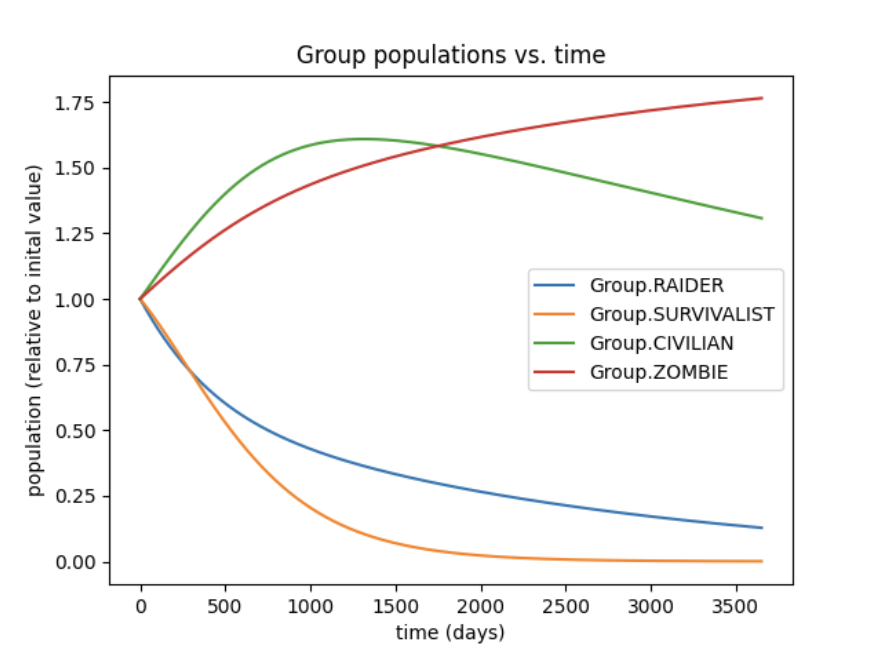
\includegraphics[width=7.5cm]{default_10_year.png}
    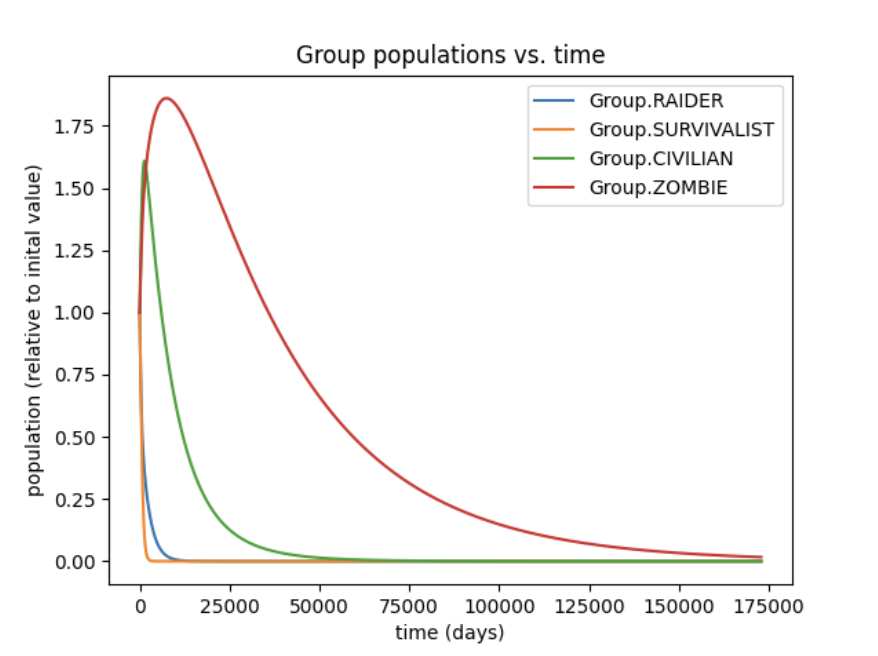
\includegraphics[width=7.5cm]{default_until_extinction.png}
    \text{Figure 2: Population sizes over time with default parameters}
\end{center}

On the left we see the first 10 years of the outbreak, and on the right we see the populations up until equilibrium. First, we can observe that the equilibrium in this scenario is extinction. This is because eventually are susceptible individuals are infected and becomes zombies, which over time die out leaving no populations left. According to the simulation, humans (susceptible individuals) would survive roughly 45000 days or approximately 123 years.

We can also observe that, in the first 10 years, the group that performs best during the apocalypse is the civilians. We see an immediate growth in population of civilians, likely due to exchanges from the survivalist group. Thereafter, all three groups asymptotically decline until extinction.

\subsection{Results: Optimistic Parameters}

We were hoping for a result in which humanity could overpower extinction and reach a shared equilibrium with the zombie population. The default parameters did not yield such a result, so we decided to tune the parameters and analyze a new result.

These new parameters we called "optimistic parameters" because they align with a world in which humanity attempts to overcome the apocalypse through teamwork and collaboration. The way we express this concept through the parameters is to set $\epsilon_{3,2} = \epsilon{2, 1} = 0$. This means that the exchanges between different susceptible groups will exclusively flow into the civilian group.

\begin{center}
    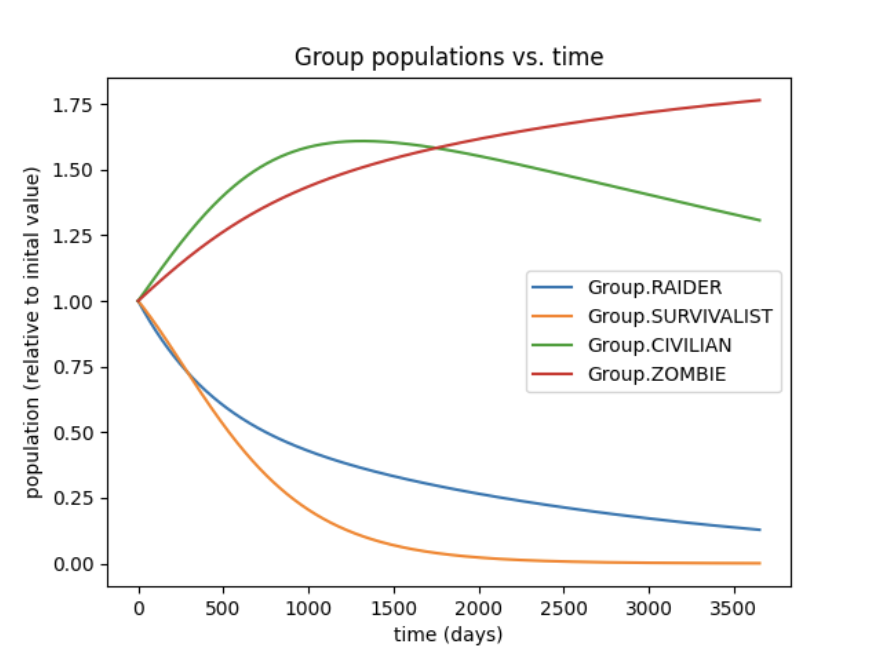
\includegraphics[width=7.5cm]{optimistic_10_year.png}
    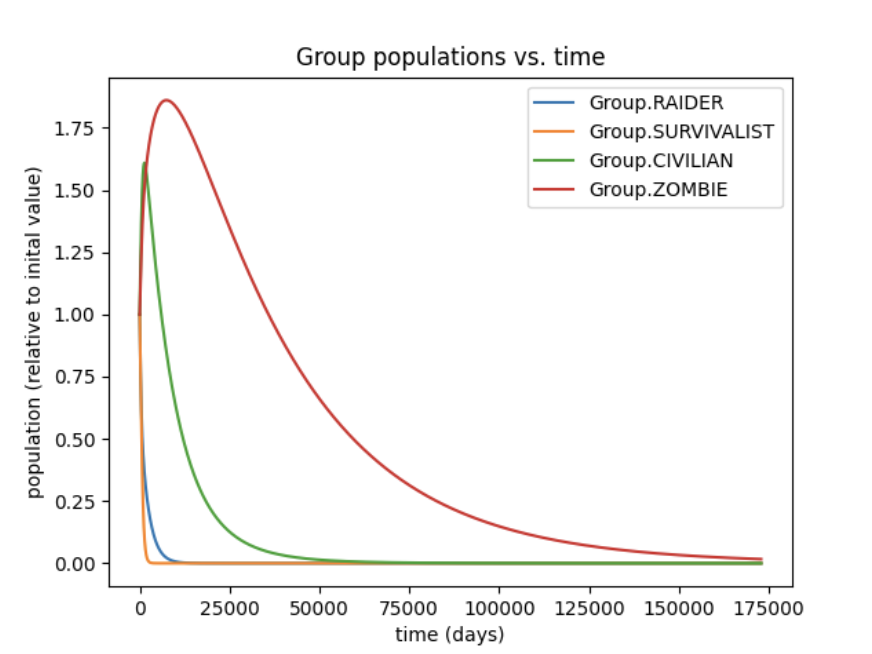
\includegraphics[width=7.5cm]{optimistic_until_extinction.png}
    \text{Figure 3: Population sizes over time with optimistic parameters}
\end{center}

Here, we can observe an even larger initial increase in the size of the civilian group. However, humanity is still completely infected by zombies and then later driven to extinction entirely. The process of extinction is elongated under these parameters, taking approximately 50000 days or approximately 136 years. This is likely due to the lower death rates and infection rates found among the civilian populations. In other words, all susceptible individuals are funnels into the civilian group, where it takes longer for them to be eradicated, explaining the elongated extinction time.

\subsection{Results: Pessimistic Parameters}

Perhaps our assumption that survival through collaboration was naive, so we also tested with a set of pessimistic parameters. These parameters are meant to encode a world in which humanity attempts to overcome the apocalypse through exploitation and self interest. The parameters are essentially the reversal of the optimistic parameters: $\epsilon_{1,2} = \epsilon{2,3} = 0$. In other words, all susceptible individuals funnel into the raiders group.

\begin{center}
    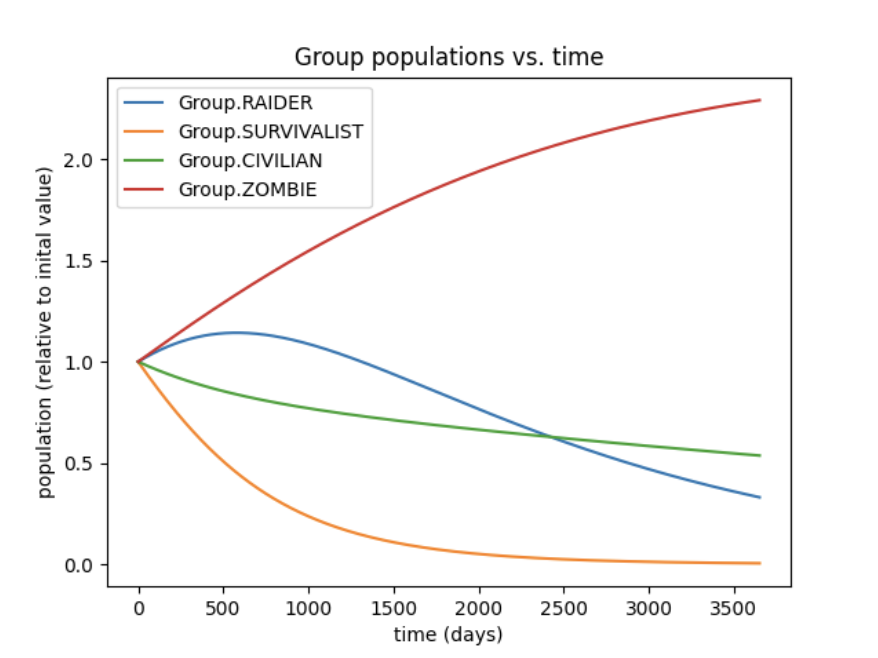
\includegraphics[width=7.5cm]{pessemistic_10_year.png}
    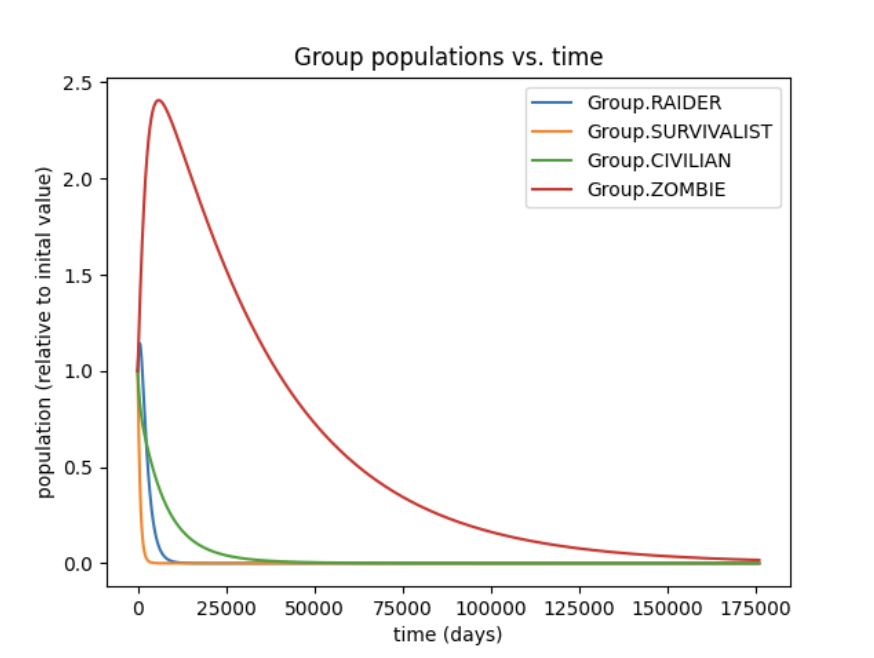
\includegraphics[width=7.5cm]{pessemistic_until_extinction.png}
    \text{Figure 4: Population sizes over time with optimistic parameters}
\end{center}

In this run of the simulation, for the first time, we can observe the raider group overtake the civilian group in terms of population. This only occurs for the first 2000 days of the simulation, about 5.5 years, before the raiders start to die out. The overall extinction time of the susceptible groups is roughly 35000 days or 96 years.

Although we were unable to find a simulation that resulted in coexistence, it is a little encouraging to see that humans performed their best against the zombie apocalypse when working together.

\section{Conclusion}

Building on and correcting ``When Zombies Attack!" led us to mathmatically analyze more recent popular culture surrounding zombie epidemics through a combination of equilibrium analysis and Monte Carlo simulation. Combining these techniques, we were able to identify the equilibria of this more complex system of four variables. Our results lead us to believe that the state of the zombie apocalypse envisioned in The Last of Us and other recent zombie media is possible. However, this state of coexistence between zombies and susceptible individuals always converges on extinction eventually.

On a lighter note, we also found that humanity was more resilient against the zombie epidemic when working together. In our simulation, we saw that through collaboration humans were able to delay the inevitable. Hence, even if the science in The Last of Us fails our models in certain cases, the show's thematic messages about the strength of community and companionship hold true.

\clearpage
\section{Appendix A: Full Simulator Code}

Below is the code full code for our simulator. It is also available on \href{https://github.com/cphalen/math2100-final-project}{GitHub}.

\begin{lstlisting}
from enum import Enum
import matplotlib.pyplot as plt
import pprint
import copy

ONE_YEAR = 365

class Group(Enum):
    RAIDER = 1
    SURVIVALIST = 2
    CIVILIAN = 3
    ZOMBIE = 4
    REMOVED = 5

class Params:
    EPSILON = 0.000001 # 10^10

    def birth_rate(group: Group):
        match group:
            case Group.RAIDER:
                return 0.000004
            case Group.SURVIVALIST:
                return 0.000001
            case Group.CIVILIAN:
                return 0.000016
            case _:
                return None

    def death_rate(group: Group):
        match group:
            case Group.RAIDER:
                return 0.0001
            case Group.SURVIVALIST:
                return 0.0003
            case Group.CIVILIAN:
                return 0.00006
            case Group.ZOMBIE:
                return 0.00003
            case _:
                return None

    def zombie_rate(group: Group):
        match group:
            case Group.RAIDER:
                return 0.0002
            case Group.SURVIVALIST:
                return 0.0004
            case Group.CIVILIAN:
                return 0.00003
            case _:
                return None
            
    def exchange_rate(src_group: Group, dest_group: Group):
        match (src_group, dest_group):
            case (Group.RAIDER, Group.SURVIVALIST):
                return 0.0009
            case (Group.SURVIVALIST, Group.RAIDER):
                return 0.0008
            case (Group.SURVIVALIST, Group.CIVILIAN):
                return 0.001
            case (Group.CIVILIAN, Group.SURVIVALIST):
                return 0.0003
            case _:
                return None

            
class Sim:

    def __init__(self):
        self.populations = {
            Group.RAIDER: 1.0,
            Group.SURVIVALIST: 1.0,
            Group.CIVILIAN: 1.0,
            Group.ZOMBIE: 1.0,
            Group.REMOVED: 0,
        }

        self.history = {}
        for group in self.populations.keys():
            self.history[group] = [self.populations[group]]

        self.printer = pprint.PrettyPrinter(indent=4)

    def step_group(self, group):
        match group:
            case Group.RAIDER:
                from_birth = Params.birth_rate(Group.RAIDER) * self.populations.get(Group.RAIDER)
                from_survivalist = Params.exchange_rate(Group.SURVIVALIST, Group.RAIDER) * self.populations.get(Group.RAIDER) * self.populations.get(Group.SURVIVALIST)
                to_survivalist = Params.exchange_rate(Group.RAIDER, Group.SURVIVALIST) * self.populations.get(Group.RAIDER) * self.populations.get(Group.SURVIVALIST)
                to_zombie = Params.zombie_rate(Group.RAIDER) * self.populations.get(Group.RAIDER) * self.populations.get(Group.ZOMBIE)
                to_removed = Params.death_rate(Group.RAIDER) * self.populations.get(Group.RAIDER)
                return from_birth + from_survivalist - to_survivalist - to_zombie - to_removed
            case Group.SURVIVALIST:
                from_birth = Params.birth_rate(Group.SURVIVALIST) * self.populations.get(Group.SURVIVALIST)
                from_raider = Params.exchange_rate(Group.RAIDER, Group.SURVIVALIST) * self.populations.get(Group.SURVIVALIST) * self.populations.get(Group.RAIDER)
                from_civilian = Params.exchange_rate(Group.CIVILIAN, Group.SURVIVALIST) * self.populations.get(Group.SURVIVALIST) * self.populations.get(Group.CIVILIAN)
                to_raider = Params.exchange_rate(Group.SURVIVALIST, Group.RAIDER) * self.populations.get(Group.SURVIVALIST) * self.populations.get(Group.RAIDER)
                to_civilian = Params.exchange_rate(Group.SURVIVALIST, Group.CIVILIAN) * self.populations.get(Group.SURVIVALIST) * self.populations.get(Group.CIVILIAN)
                to_zombie = Params.zombie_rate(Group.SURVIVALIST) * self.populations.get(Group.SURVIVALIST) * self.populations.get(Group.ZOMBIE)
                to_removed = Params.death_rate(Group.SURVIVALIST) * self.populations.get(Group.SURVIVALIST)
                return from_birth + from_raider + from_civilian - to_raider - to_civilian - to_zombie - to_removed
            case Group.CIVILIAN:
                from_birth = Params.birth_rate(Group.SURVIVALIST) * self.populations.get(Group.CIVILIAN)
                from_survivalist = Params.exchange_rate(Group.SURVIVALIST, Group.CIVILIAN) * self.populations.get(Group.CIVILIAN) * self.populations.get(Group.SURVIVALIST)
                to_survivalist = Params.exchange_rate(Group.CIVILIAN, Group.SURVIVALIST) * self.populations.get(Group.CIVILIAN) * self.populations.get(Group.SURVIVALIST)
                to_zombie = Params.zombie_rate(Group.CIVILIAN) * self.populations.get(Group.CIVILIAN) * self.populations.get(Group.ZOMBIE)
                to_removed = Params.death_rate(Group.CIVILIAN) * self.populations.get(Group.CIVILIAN)
                return from_birth + from_survivalist - to_survivalist - to_zombie - to_removed
            case Group.ZOMBIE:
                from_raider = Params.zombie_rate(Group.RAIDER) * self.populations.get(Group.ZOMBIE) * self.populations.get(Group.RAIDER)
                from_survivalist = Params.zombie_rate(Group.SURVIVALIST) * self.populations.get(Group.ZOMBIE) * self.populations.get(Group.SURVIVALIST)
                from_civilian = Params.zombie_rate(Group.CIVILIAN) * self.populations.get(Group.ZOMBIE) * self.populations.get(Group.CIVILIAN)
                to_removed = Params.death_rate(Group.ZOMBIE) * self.populations.get(Group.ZOMBIE)
                return from_raider + from_survivalist + from_civilian - to_removed
            case Group.REMOVED:
                from_raider = Params.death_rate(Group.RAIDER) * self.populations.get(Group.RAIDER)
                from_survivalist = Params.death_rate(Group.SURVIVALIST) * self.populations.get(Group.SURVIVALIST)
                from_civilian = Params.death_rate(Group.CIVILIAN) * self.populations.get(Group.CIVILIAN)
                from_zombie = Params.death_rate(Group.ZOMBIE) * self.populations.get(Group.ZOMBIE)
                return from_raider + from_survivalist + from_civilian + from_zombie
            
    def step(self):
        updates = {}

        # simulate all of these transformations happening simultaneous
        for group in self.populations.keys():
            new_population = self.step_group(group)
            updates[group] = new_population

        # update state with new population values
        for group in updates.keys():
            self.populations[group] += updates[group]
            self.populations[group] = max(self.populations[group], 0)
            self.history[group].append(self.populations[group])

    def simulate(self, limit=None):
        i = 0
        while True:
            old_populations = copy.copy(self.populations)
            self.step()

            diff = 0
            i += 1
            for group in old_populations.keys():
                diff += abs(self.populations.get(group) - old_populations.get(group))

            if diff < Params.EPSILON or (limit is not None and i >= limit):
                print(i)
                return

    def print(self):
        self.printer.pprint(self.populations)
        total = 0
        for value in self.populations.values():
            total += value
        print(total)


    def plot(self):
        for group, history in self.history.items():
            if group == Group.REMOVED:
                # we don't need to display the removed
                continue
            plt.plot(list(range(len(history))), history, label=str(group), markersize=1)

        plt.xlabel('time (days)')
        plt.ylabel('population (relative to inital value)')
        plt.title('Group populations vs. time')
        plt.legend()

        plt.show()


if __name__ == "__main__":
    sim = Sim()
    sim.simulate()
    sim.print()
    sim.plot()
\end{lstlisting}

\end{document}